% Chapter 1

\chapter{Introduction}
\label{Chap1}

\lhead{Chapter 1. \emph{Introduction}}
\begin{figure}
    \centering
    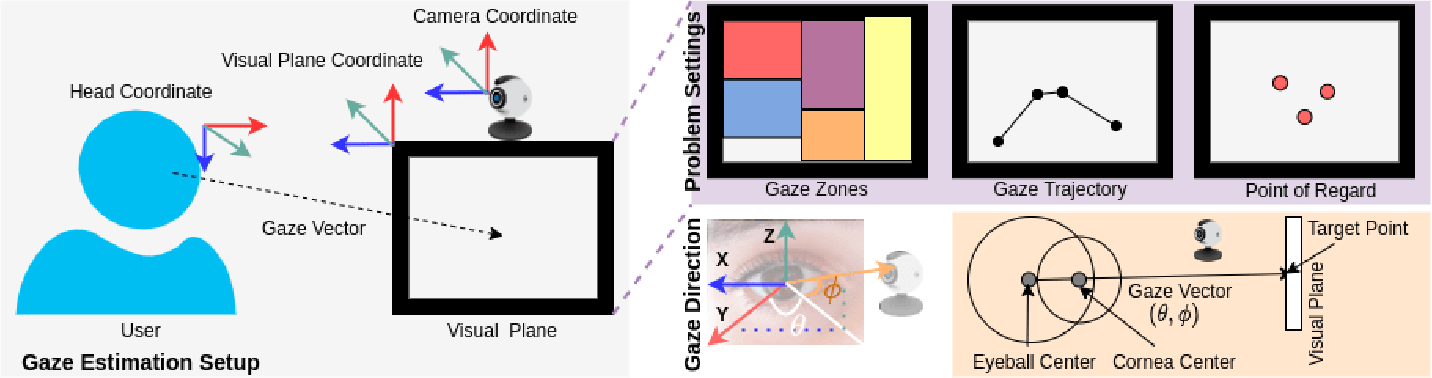
\includegraphics[width=\textwidth,height=5cm]{img/figures/gaze_estimation_setup.png}
    \caption{Overview of Gaze-Estimation setups. Recovered from \cite{survey_automatic_gaze_ghosh}}
    \label{gaze_estimation_setup}
 \end{figure}


\section{Gaze-Tracking}
Applications of estimating the human eye gaze direction, or Gaze-Tracking, can be found in multiple study areas such as health care \cite{EyeTrackMedical}, virtual-reality \cite{EyeVR}, and human-computer interaction \cite{Gaze-Controlled-Web}. Devices that utilize gaze-tracking methods for human-computer interaction are often referred to as Eye Trackers. While there is commercial use for Eye Trackers, they have not reached the accuracy needed to allow users with fine-motor disabilities to interact with a computer by using their own eyes as a replacement for a traditional mouse device.

Conventional methods for gaze-tracking require additional devices such as infrared light in order to make the gaze estimations. However, these methods are prone to error in poor light conditions.

Research in computer vision and Deep Learning have allowed improvement in Gaze-Tracking systems by allowing better predictions while also being less intrusive for users with no additional devices required.


\begin{figure}
    \centering
    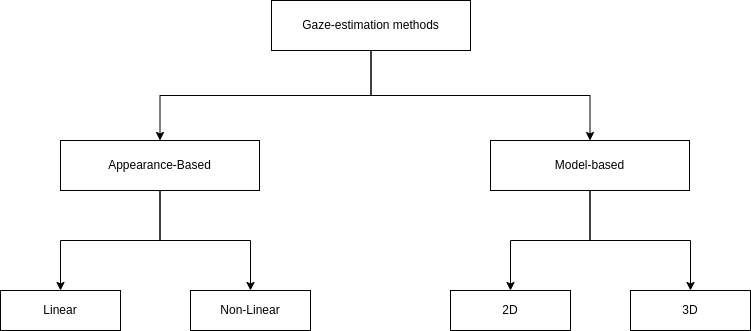
\includegraphics[scale=0.6]{img/figures/methods_classification.png}
    \caption{Overview classification of Gaze-Tracking methods }
    \label{GEClassification}
 \end{figure}


Gaze-Tracking with computer vision can be achieved with two different type of methods: Model-based methods and Appearance-based methods. These methods will be described in the following sections.

\section{Model-based methods}
Model-based methods, or sometimes referred to as feature-based methods, use the geometric form of the eyes to make the eye gaze prediction.
As seen on \autoref{GEClassification}, these can be interpreted as 3D models. Model-based 3D Gaze-Estimation
methods use 3D eyeball models and estimate the gaze direction using geometric eye features, such as the iris center and the eye corners \cite{general_theory_remote_gaze_3d_model}.

Furthermore, most these methods require an infrared light source (IR) in order to create a refraction in the human eye which is then used to calculate the eye gaze direction by comparing the refraction position with the pupil position. The main drawback of model-based methods is that they can have a lower accuracy with low-resolution images and poor-condition lighting environments. Additionally, all of them have limited working distance.1

Some state-of-the-art commercial products that have adapted these techniques are Tobii Eye Tracker (\url{https://www.tobii.com/}), Eye Tribe (\url{https://imotions.com/hardware/the-eye-tribe-tracker/}) and EyeSee (\url{https://eyesee-research.com/}). 
While these products allow very accurate predictions for the Eye Tracking, they suffer from the previously mentioned model based methods disadvantages while also requiring users to purchase additional expensive equipment. Most Eye-Tracking products also require wearable glasses peripherals that can be intrusive for daily usage. 

With the increase of interest and usage of Gaze-Tracking, there is also a growing need for new Eye-Trackers that are cheap and easy to use.
Gaze-Tracking methods that utilize built-in or external cameras included in almost every computer can be used as a way of making eye tracking more accessible. Appearance-based approaches are beginning to be researched to achieve the previous goal.

\section{Appearance-based methods}
Recently, investigations for appearance based methods with Deep Learning has surfaced which have demonstrated high accuracy while only using on-the-shelf web cameras to capture the human eye appearance hence the method name.

Conventional appearance-based methods used regression in order to learn the mappings from appearance to human gaze. However, since these methods use the appearance of the eye, the main challenges are head motion and subject differences that alter the eye appearance on use.

To overcome the previous challenges, appearance-based Gaze-Estimation with Deep Learning has become a trend in research. Deep Learning based methods can extract high-level abstract gaze features from high-dimensional images, making them more robust and accurate than conventional methods. The mapping between eye-images and gaze direction can be achieved with various regression techniques, such as neural networks, local interpolation, or Gaussian process regression. Convolutional Neural Networks (CNNs) models are commonly used in computer vision tasks for its high accuracy and performance. 
Current state-of-the-art solutions have begun to adopt CNN based architectures, adopting the advantages of appearance-based methods and achieving high accuracy. CNN models used for Gaze-Tracking learn from RGB images which are preprocessed to segment the human eyes in training.

Some of the drawbacks that appearance-based methods have been that they require more images for training than model-based methods, which are not easily retrieved. Additionally, since most appearance-based methods require deep-learning architectures such as Convolutional Neural Networks, they require higher computational power for training. Several works apply CNNs for gaze estimation, as they have shown to outperform traditional model-based approaches \cite{GazeEstimationInTheWild}.

% Chapter 2

\chapter{State-of-the-art}
\label{Chap2}

\lhead{Chapter 2. \emph{State-of-the-art}}

\section{Related Work}

\begin{figure}
    \centering
    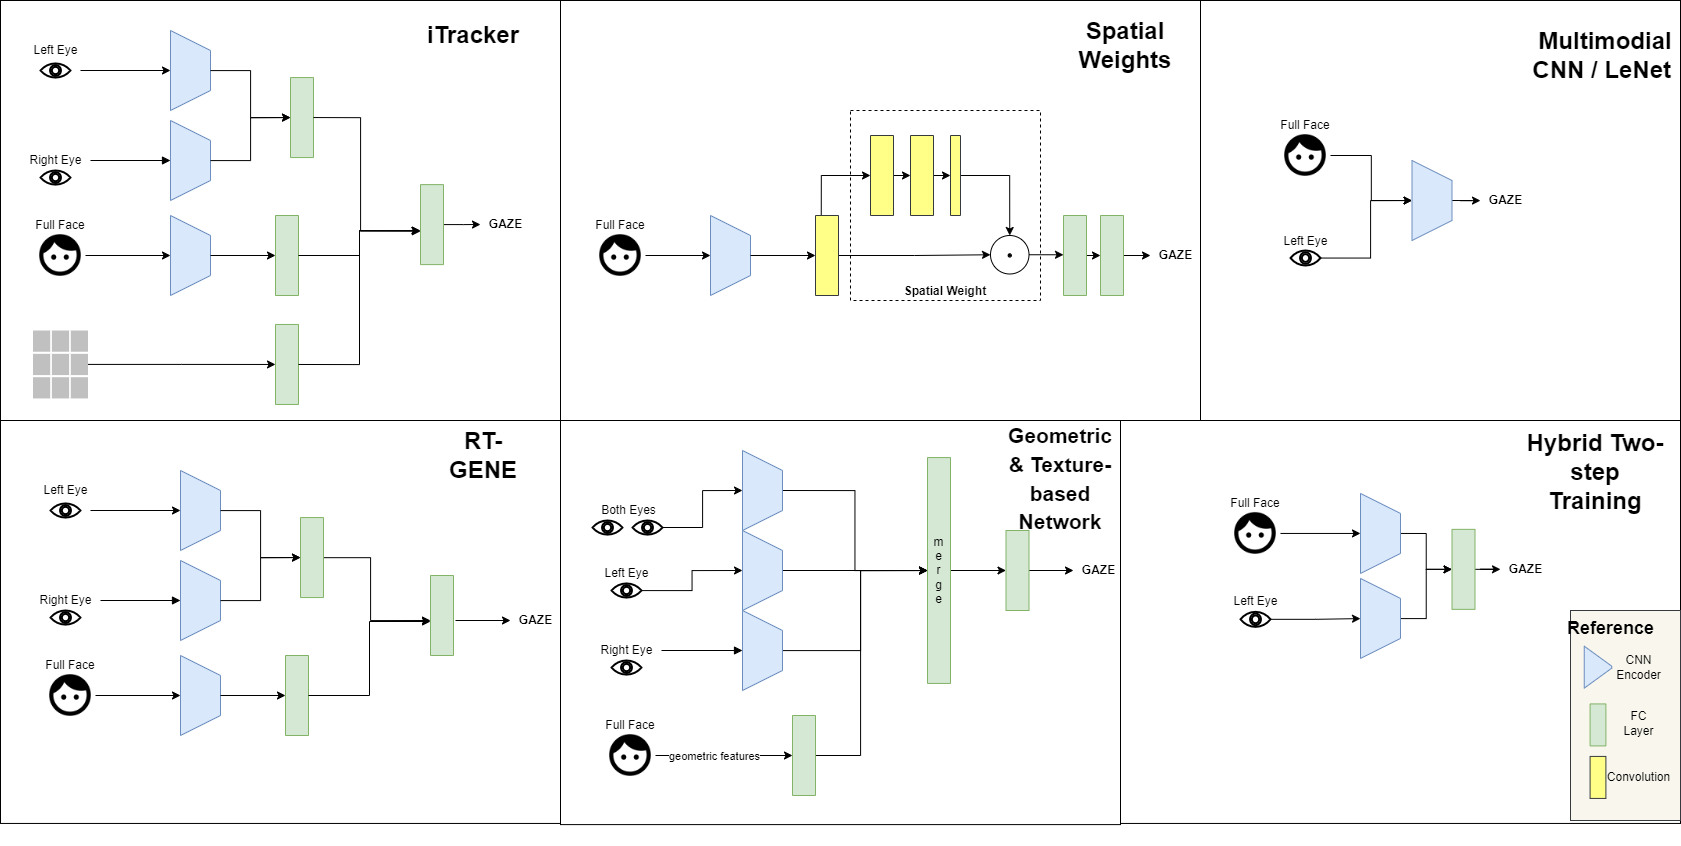
\includegraphics[width=\textwidth,height=9cm]{img/figures/gaze-architectures.png}
    \caption{Generalized architectures of state-of-the-art models}
    \label{architectures_comparison}
 \end{figure}

 \begin{table}[h!]
    \caption{State-of-the-art architecture comparison}
    \centering
    \label{tab:architectures}
    \begin{tabular}{c c c c c c}
    \hline\hline
    Name & Datasets used \# & Angular Error & Euclidean Error & Year & Reference \# \\
    \hline\hline
        GazeCapture & 2,500,000 & 136 & 1500 & 13 \\
        MMPIIGaze & 213,659 & 2.1 & 15 & 20 \\
        CAVE & 5,880 & 2.2 & 56 & 105 \\
        ETH-XGaze & 1,083,492 & 123 & 110 & 600 \\ [1ex]
    \hline
    \end{tabular}
\end{table}

\subsection{Multimodal Convolutional Neural Network}
Zhang et al. proposed a six-layered CNN based on LeNet that takes the eye image as input and combines the head pose in the last fully connected layer of the network \cite{GazeEstimationInTheWild}. The results demonstrated a large performance gap between person-specific training results (RF model) with the proposed CNN model and revealed the potential of appearance-based gaze estimation.

\subsection{Spatial Weight CNN}
After the previous proposal, Zhang et al. proposed a spatial weights CNN based on the AlexNet architecture \cite{alex_net} that takes the full face image as input \cite{written_all_over_your_face}. The spatial weights classify the importance of different facial areas in order to perform the Gaze-Estimation. This mechanism includes three additional 1 x 1 convolutional layer followed by a ReLU activation. Compared to other approaches only use eye regions, this method was demonstrated to be more robust against appearance variation such as head pose as well as illumination. The results achieved an error of ~4.8-6.0$^{\circ}$.

\subsection{iTracker}
Kannan et al. proposed a CNN architecture for an iOS based Gaze-Tracking system called iTracker \cite{iTracker}. The model's large neural network was constructed with multiple smaller neural networks, with four total inputs: a right eye image, a left eye image, a face image, and a face-grid. The face-grid is a 25x25 binary grid that indicates where the user face is placed relatively to the camera view. 

This model achieved 1.66 centimeter error with no calibration needed. The GazeCapture dataset which is described in \autoref{state-art-datasets} was used to train this model.

While achieving good results, this model is biased with mobile usage which makes it unusable for laptop or computer desktop usage. Additionally, the authors describe there being room for improvement for better segmentation of eyes. However, by adjusting the model's face-grid dimensions to simulate webcam dimensions and with a different dataset, the model could potentially be used for desktop/laptop use.

\subsection{Geometric \& Texture-based Networks}
Jyoti et al. proposed an ensemble of networks that uses the full face, left and right eye \cite{jyoti_automatic_2018}.
A Deep Neural Network (DNN) is trained using the face geometric features. Secondly, three CNNs are trained for the texture based features i.e. the segment of the left eye, right eye, and the combined eyes. The model was trained with the publicly available Columbia Eye Gaze and TabletGaze datasets for experiments. When trained with the Columbia Eye Gaza dataset, experiments resulted in an error of 2.22$^{\circ}$. Additionally, the authors emphasize on the importance of choosing
different activation functions for different results by comparing the model outcome with ReLU vs Swish, where the former achieved better performance for geometric network while Swish showed better performance on the rest.

\subsection{RT-GENE}
Fischer et al. proposed a two-stream VGG network that takes the left and right as inputs \cite{fischer_rt-gene_2018}. This approach considers large camera-to-user distances and high variations in head pose found in natural environments. This approach allows automatic annotation of subject's ground truth gaze and head pose regardless of large camera-user distances, achieving an error of 7.7$^{\circ}$. However, the approach setup requires additional devices such as mobile eye-tracking glasses (Kinect v2 RGB-D camera).

\subsection{Hybrid Two-step Training}
Deng and Zhu proposed a two-step training architecture, where a head CNN and eye CNN are independently trained and then together transformed with a "gaze transform layer" \cite{deng_monocular_2017}. The proposed model does not suffer from head-gaze correlation overfitting which makes it possible to use existing datasets for training. The solution achieves an error of 5.6$^{\circ}$ when trained with a large dataset, achieving state-of-the-art gaze tracking accuracy. 

\section{Datasets}
\label{state-art-datasets}


\begin{figure}
    \centering
    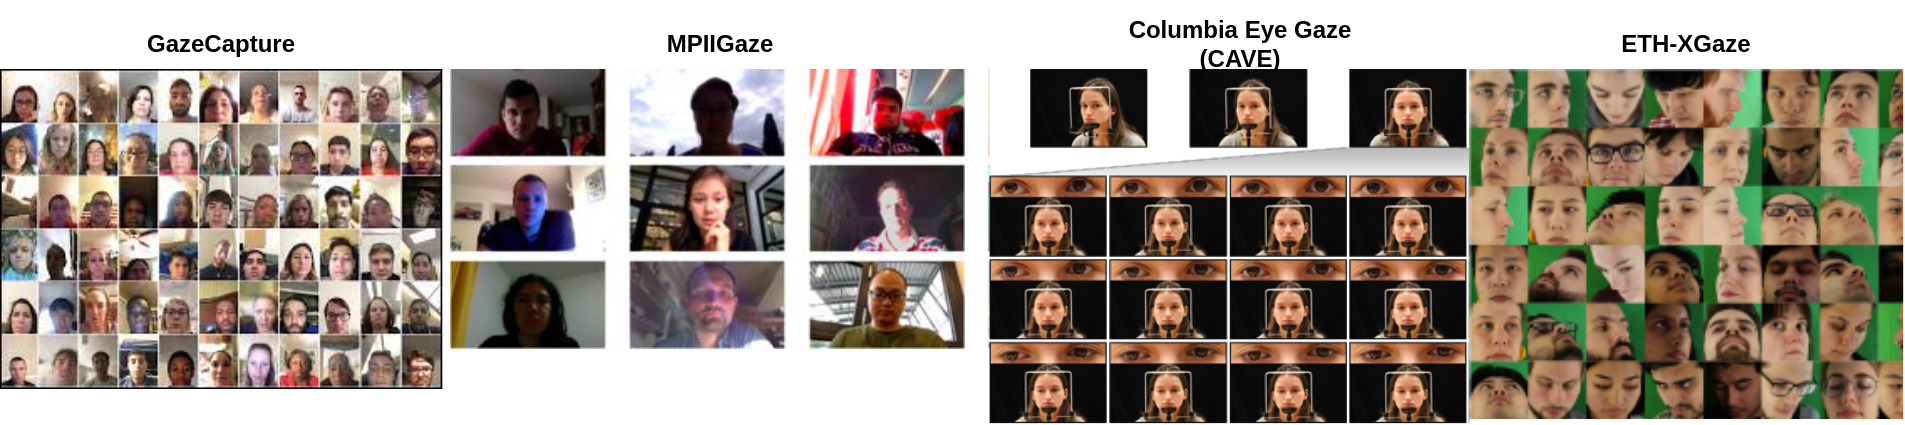
\includegraphics[width=\textwidth,height=4cm]{img/figures/datasets.png}
    \caption{Samples from different datasets. Recovered from \cite{GazeCapture}, \cite{GazeEstimationInTheWild}, \cite{CAVE_0324} and \cite{Zhang2020ETHXGaze} respectively. }
    \label{Datasets}
 \end{figure}

 \begin{table}[h!]
    \caption{Dataset comparison}
    \centering
    \label{tab:dataset}
    \begin{tabulary}{\textwidth}{LCCCCCCCC}
        \hline
        Dataset & Total Images \# & Size (GB) & Subjects \# & Gaze Points \# & Full Face & 2D Gaze & 3D Gaze & Ref \\
        \hline
        GazeCapture 2016 & 2.4M & 136 & 1,474 & 203 & \cmark & \cmark & \xmark & \cite{GazeCapture} \\
        \hline
        MPIIGaze 2015 & 213K & 2.1 & 15 & 203 & \xmark & \cmark & \cmark & \cite{GazeEstimationInTheWild} \\
        \hline
        CAVE 2013 & 6K & 2.2 & 56 & 105 & \cmark & \xmark & \cmark & \cite{CAVE_0324} \\
        \hline
        ETH-XGaze 2020 & 1.1M & 123 & 110 & 600 & \cmark & \cmark & \cmark & \cite{Zhang2020ETHXGaze} \\
        \hline
        \end{tabulary}
\end{table}

Until recently, datasets for Gaze-Estimation models training were built manually by taking pictures of different users' faces by placing their head firmly in a stand. Training models require multiple high-quality images, which makes the previous methods slow and not ideal.
To improve the previous methods' problem, multiple data sets containing images for eye tracking have been compiled with crowd founding to train new models.
\autoref{Datasets} represents an overview of different state-of-the-art datasets, while \autoref{tab:dataset} provides an analytical comparison of each of them.

\subsection{GazeCapture}
Krafka et al. built and released the GazeCapture dataset, which crowdfunded a mobile-based data set of approximately 1500 participants from a wide variety of backgrounds captured by an iOS application \cite{GazeCapture}. However, given that this dataset is built with mobile users, training with this dataset may lead to a huge bias towards mobile users which could lead to poor results with laptop or desktop use.
Additionally, the authors provide pre-trained models utilizing the dataset available as open source (\url{https://github.com/CSAILVision/GazeCapture}).

\subsection{MMPIIGaze}
Another state-of-the-art dataset that has been widely used is the MMPIIGaze dataset created by Zhang et al. \cite{GazeEstimationInTheWild}.
The dataset contains a total of 213,659 images from 15 participants. For each participant, there is a varied number of
images ranging from 34,745 to 1,498. The dataset contains multiple features, our target being the 3D gaze target position related to camera.
The dataset is taken from the participant's laptops, contrasting GazeCapture's images taken from mobile devices.

\subsection{Columbia Eye Gaze / CAVE}
The CAVE dataset \cite{CAVE_0324} consists of 5,880 images of 56 different participants. For each participant, there are 5 head poses with 21 gaze directions per head pose. The authors describe the dataset as having more fixed gaze targets than other publicly available gaze datasets. The participants are ethnically diverse and some of them are captured wearing glasses which makes this a strong candidate for learning. The dataset comes with already-segmented eye areas, so segmentation step can be skipped.

\subsection{ETH-XGaze}
Finally, the ETH-XGaze dataset \cite{Zhang2020ETHXGaze} consists of over 1,000,000 images of varying gaze under extreme head posers collected from 110 participants While the extreme varied head poses provide good opportunities for learning, for the case of this project the head poses that are not looking into the screen would not be useful so hey must be discarded.

\subsection{Discussion}
As seen on \autoref{tab:dataset}, the dataset with the biggest scale is ETH-XGaze, having the biggest samples and gaze points available. 
While training with the ETH-XGaze dataset would create the biggest model, the huge size of its collection of images might require high computational
power and training time in order to fully train the model. While GazeCapture is also a great candidate, its small number of gaze points 
is insufficient for the purpose of gaze-estimation in a computer screen.

\chapter{Development}
\label{Chap3}
\lhead{Chapter 3. \emph{Development}}


\section{Objectives}
For this research, a new proposed model for Gaze-Estimation that outperforms current state-of-the art systems is 
the goal. To fully realize this, the model must have lower accuracy and higher speed.
Accuracy can be determined with evaluation metrics described in \autoref{EvaluationMetrics}, while the speed of the model
must be fast enough in order to potentially use this gaze-estimation system in real-time on the average user computer.

\section{Evaluation Metrics}
\label{EvaluationMetrics}
There are two commonly used metrics for performance evaluation in Gaze-Tracking Systems:
Euclidean distance and the angular error. Angular error is used when referring to 3D gaze estimation, while euclidean distance is used for 2D gaze estimation.

Assuming the gaze direction is \boldmath $g \in \mathbb{R}^3$, and the estimated gaze direction is
\boldmath $\hat{g}  \in \mathbb{R}^3$, the angular error can be calculated with the formula:

\begin{equation} \iota _{angular} = \frac{g \cdot  \hat{g} }{ \|g\|\|\hat{g}\| } \end{equation}

For 2D gaze estimation, the actual gaze position is denoted as 
\boldmath $p \in \mathbb{R}^2$ while the estimated gaze position as
\boldmath $\hat{g} \in \mathbb{R}^2$. This would result in the following formula:

\begin{equation} \iota _{Euclidean} = \| p - \hat{p} \|  \end{equation}

For the purpose of this research, given that the gaze prediction desired is of the screen coordinates that the user is looking at, euclidean distance will be used
as a performance evaluation metric for the proposed model's 2D gaze estimation.

\section{Proposed Architecture}

\section{Training}

\chapter{Results}
\label{Chap4}
\lhead{Chapter 4. \emph{Results}}


\chapter{Conclusion}
\label{Chap5}
\lhead{Chapter 5. \emph{Conclusion}}
